% =============================================================================
%  SoSa -- boş şablon / blank starting point.  Copy this file and fill it in.
%  Derleme / compile twice:  latexmk -pdf skeleton.tex
% =============================================================================
\documentclass[ornament=alternate,fontsize=11,lang=turkish]{sosa}

% --- süsleme şeritleri / ornament strips -------------------------------------
\SosaOrnamentCycle{%
  assets/ornaments/ornament-01,%
  assets/ornaments/ornament-02,%
  assets/ornaments/ornament-03%
}
\SosaHero{assets/hero/hero-01}

% --- künye / running heads ---------------------------------------------------
\SosaStartPage{1}
\SosaMasthead{Sosyal Bilimler ve Sağlık Bülteni (SoSa). 2026; Bahar(18):1-12}
\SosaRunningHead{Kısa başlık. SoSa. 2026;Bahar(18)}

% --- başlık sayfası / front matter -------------------------------------------
\SosaArticleType{Özgün Makale}
\SosaTitleTR{Makalenin Türkçe Başlığı}
\SosaTitleEN{English Title of the Article}

\author{%
  Ad Soyad\sosaaff{1}\orcid{0000-0000-0000-0000},
  Ad Soyad\sosaaff{2}\orcid{0000-0000-0000-0001}%
}
\SosaAffiliations{%
  \item Unvan, Kurum, Bölüm, Şehir, Türkiye.
  \item Unvan, Kurum, Bölüm, Şehir, Türkiye.%
}

\SosaOz{%
  \textbf{Giriş:} \ldots

  \textbf{Gereç-Yöntem:} \ldots

  \textbf{Bulgular:} \ldots

  \textbf{Sonuç-Öneriler:} \ldots%
}
\SosaKeywordsTR{birinci, ikinci, üçüncü}

\SosaAbstract{%
  \textbf{Introduction:} \ldots

  \textbf{Materials and Methods:} \ldots

  \textbf{Results:} \ldots

  \textbf{Conclusion and Recommendations:} \ldots%
}
\SosaKeywordsEN{first, second, third}

\SosaReceived{00.00.2026}
\SosaAccepted{00.00.2026}
\SosaPublished{00.00.2026}
\SosaCorrespondingAuthor{Ad Soyad}
\SosaCorrespondingEmail{ad.soyad@kurum.edu.tr}
\SosaHandlingEditor{Ad Soyad}
\SosaCitation{Soyad, A., \& Soyad, B. (2026). Makalenin Türkçe Başlığı.
  \textit{Sosyal Bilimler ve Sağlık Bülteni (SoSa), BAHAR(18),} 1-12}

% =============================================================================
\begin{document}
\maketitle

\section{Giriş}

Metin buraya.

\section{Gereç-Yöntem}

Metin buraya.

\section{Bulgular}

% Sayfa genişliğinde tablo -- sosawide, o sayfanın süslemesini de kaldırır.
% A full-width table -- sosawide also drops that page's ornament strip.
\begin{table}[!ht]
\begin{sosawide}
  \caption{Tablo başlığı}
  \label{tab:ornek}
  \centering
  \begin{sosatabular}[\sosatablesmall]{@{}L{150pt}L{130pt}R{110pt}@{}}
    \textbf{Değişkenler} & & \textbf{Sayı (\%)} \\
    \midrule
    Satır & Alt kırılım & 000 (\%00,0) \\
  \end{sosatabular}
\end{sosawide}
\end{table}

% Normal genişlikte tablo / a table that fits the ornament measure
\begin{table}[!ht]
  \caption{Tablo başlığı}
  \begin{sosatabular}{@{}L{170pt}L{90pt}R{140pt}@{}}
    \textbf{Değişkenler} & & \textbf{Sayı (\%)} \\
    \midrule
    Satır & Alt kırılım & 000 (\%00,0) \\
  \end{sosatabular}
\end{table}

\begin{figure}[!ht]
  \centering
  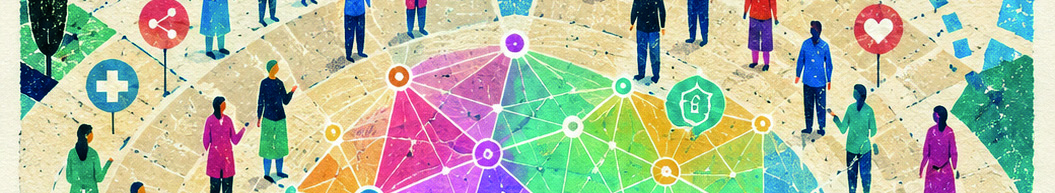
\includegraphics[width=0.6\textwidth]{assets/hero/hero-01}
  \caption{Görsel başlığı}
\end{figure}

\section{Tartışma}

\begin{quote}
Alıntı metni buraya. (K1)
\end{quote}

\section{Sonuç ve Öneriler}

Metin buraya.

\begin{sosareferences}

Soyad, A. (2025). Makale başlığı. \textit{Dergi Adı, 7}(3), 193.
\url{https://doi.org/10.0000/00000}

Soyad, B., \& Soyad, C. (2024). Kitap başlığı. Yayınevi.

\end{sosareferences}

\end{document}
